\documentclass[12pt,]{article}
\usepackage{lmodern}
\usepackage{amssymb,amsmath}
\usepackage{ifxetex,ifluatex}
\usepackage{fixltx2e} % provides \textsubscript
\ifnum 0\ifxetex 1\fi\ifluatex 1\fi=0 % if pdftex
  \usepackage[T1]{fontenc}
  \usepackage[utf8]{inputenc}
\else % if luatex or xelatex
  \ifxetex
    \usepackage{mathspec}
    \usepackage{xltxtra,xunicode}
  \else
    \usepackage{fontspec}
  \fi
  \defaultfontfeatures{Mapping=tex-text,Scale=MatchLowercase}
  \newcommand{\euro}{€}
\fi
% use upquote if available, for straight quotes in verbatim environments
\IfFileExists{upquote.sty}{\usepackage{upquote}}{}
% use microtype if available
\IfFileExists{microtype.sty}{%
\usepackage{microtype}
\UseMicrotypeSet[protrusion]{basicmath} % disable protrusion for tt fonts
}{}
\usepackage[margin=1in]{geometry}
\usepackage{graphicx}
\makeatletter
\def\maxwidth{\ifdim\Gin@nat@width>\linewidth\linewidth\else\Gin@nat@width\fi}
\def\maxheight{\ifdim\Gin@nat@height>\textheight\textheight\else\Gin@nat@height\fi}
\makeatother
% Scale images if necessary, so that they will not overflow the page
% margins by default, and it is still possible to overwrite the defaults
% using explicit options in \includegraphics[width, height, ...]{}
\setkeys{Gin}{width=\maxwidth,height=\maxheight,keepaspectratio}
\ifxetex
  \usepackage[setpagesize=false, % page size defined by xetex
              unicode=false, % unicode breaks when used with xetex
              xetex]{hyperref}
\else
  \usepackage[unicode=true]{hyperref}
\fi
\hypersetup{breaklinks=true,
            bookmarks=true,
            pdfauthor={Kyle MacDonald; Todd LeMarr; David Corina; Virginia Marchman; Anne Fernald},
            pdftitle={Age-related changes in children's real-time American Sign Language comprehension},
            colorlinks=true,
            citecolor=blue,
            urlcolor=blue,
            linkcolor=magenta,
            pdfborder={0 0 0}}
\urlstyle{same}  % don't use monospace font for urls
\setlength{\parindent}{0pt}
\setlength{\parskip}{6pt plus 2pt minus 1pt}
\setlength{\emergencystretch}{3em}  % prevent overfull lines
\setcounter{secnumdepth}{0}

%%% Use protect on footnotes to avoid problems with footnotes in titles
\let\rmarkdownfootnote\footnote%
\def\footnote{\protect\rmarkdownfootnote}

%%% Change title format to be more compact
\usepackage{titling}

% Create subtitle command for use in maketitle
\newcommand{\subtitle}[1]{
  \posttitle{
    \begin{center}\large#1\end{center}
    }
}

\setlength{\droptitle}{-2em}
  \title{Age-related changes in children's real-time American Sign Language
comprehension}
  \pretitle{\vspace{\droptitle}\centering\huge}
  \posttitle{\par}
  \author{Kyle MacDonald \\ Todd LeMarr \\ David Corina \\ Virginia Marchman \\ Anne Fernald}
  \preauthor{\centering\large\emph}
  \postauthor{\par}
  \date{}
  \predate{}\postdate{}



\begin{document}

\maketitle

\begin{abstract}
Children learning sign language must use vision to process linguistic
information \emph{and} to attend to objects in the world, creating a
challenge for young learners' real-time language comprehension.
Extensive research with children learning spoken language shows that the
ability to interpret speech in real time with high efficiency is
critical to language development (Fernald \& Marchman, 2012). But we
know relatively little about how visual language learners develop this
critical language skill. This cross-sectional study develops the first
measures of real-time American Sign Language (ASL) comprehension
abilities, and explores links between these skills and children's
vocabulary development. 29 native ASL-learners (16-53 mos) and 19 fluent
adult signers completed a novel measures of ASL processing efficiency.
Children's comprehension skills improved with age, and adult signers
were more efficient than children. Importantly, children's processing
skills strongly correlated with their vocabulary size, providing
evidence that the ability to efficiently establish reference in
real-time is linked to meaningful linguistic outcomes. These novel
findings show that visual language learners, like children learning
spoken languages, make impressive gains in the efficiency of language
interpretation over the first few years of life as they progress towards
adult-like levels of fluency.
\end{abstract}

\newpage

\section{Introduction}\label{introduction}

Understanding language rapidly and accurately is central to our ability
to function effectively in daily life. One fundamental component of
language understanding is establishing reference: linking abstract
symbols (i.e.~words and signs) to concrete objects in the
world.\footnote{This problem is also known as referential uncertainty
  (Quine, 1960): that a speaker's utterance could refer to many possible
  objects in the visual scene, to parts of of those objects, or even to
  something that is not present.} While children learning spoken
languages can simultaneously attend to objects and listen to their
caregivers, children learning American Sign Language (ASL) must rely on
vision to both look at objects and to process linguistic information.
This dual functionality requires children to disengage from the source
of language to seek out the named object, increasing the likelihood of a
mapping error or potentially creating a situation where subsequent
linguistic information is missed. Thus it is critical to understand how
young ASL users learn to efficiently establish reference during
real-time language understanding. In the current work, we aim to develop
the first measures of young ASL-learners' real-time language
comprehension skills, and we explore links between these skills and
children's age and vocabulary development.

\subsubsection{Spoken language
processing}\label{spoken-language-processing}

To follow a typical conversation, skilled listeners must rapidly
apprehend meaning in combinations of words from moment to moment as the
speech signal unfolds at rates of 10-15 phonemes/second. Extensive
research with adults using online measures\footnote{Here online measures
  refer to measuring participants' eye movements during language
  comprehension in order to provide a rapid and detailed metric for
  determining the target of their visual attention.} shows that skilled
listeners can identify spoken words before their acoustic offset,
evaluating hypotheses about word identity incrementally based on what
they have heard up to that moment, typically within 150 ms of word onset
(Marslen-Wilson \& Zwitserlood, 1989). Moreover, adults are adept in the
parallel processing of multiple streams of information, rapidly
integrating the acoustic speech signal as it unfolds in time with
information from the visual scene to derive intended meaning (Altmann \&
Kamide, 1999; Dahan \& Tanenhaus, 2004; Tanenhaus, Spivey-Knowlton,
Eberhard, \& Sedivy, 1995).

Over the past fifteen years, research with infants and young children
has incorporated the same high-resolution measures of language
processing (Fernald, Pinto, Swingley, Weinbergy, \& McRoberts, 1998;
Snedeker \& Trueswell, 2004), making it possible to obtain continuous
measures of speed and accuracy that enable sensitive assessment of
efficiency in spoken language processing even by very young children.
Using these procedures, researchers have found systematic age-related
changes in the speed and accuracy of responses to familiar words
(Fernald et al., 1998), and that efficiency in word recognition is
correlated with both individual differences in vocabulary knowledge
(Fernald, Swingley, \& Pinto, 2001; Zangl, Klarman, Thal, Fernald, \&
Bates, 2005) as well as faster rates of vocabulary growth across the
second year (Fernald, Perfors, \& Marchman, 2006). While studies have
also found associations between faster word recognition and more
advanced linguistic development in both English (Fernald et al., 2001;
Zangl \& Fernald, 2007) and Spanish (Hurtado, Marchman, \& Fernald,
2008; Lew-Williams \& Fernald, 2007), this is the first study to adapt
these online processing efficiency measures to be used with children
learning ASL.

\subsubsection{ASL processing with
adults}\label{asl-processing-with-adults}

ASL is a visual-gestural language expressed with hands, arms and face, a
modality difference with potential consequences for how linguistic
information is processed. In many ways, language processing appears to
be parallel in spoken and manual modalities. Signers show effects of:
(a) lexicality, response times to identify non-signs are slower than for
actual signs (D. P. Corina \& Emmorey, 1993)), (b) frequency, high
frequency signs are recognized faster than low frequency signs
(Carreiras, Guti{é}rrez-Sigut, Baquero, \& Corina, 2008), and (c)
phonological parameters, the sublexical units of sign -- handshape,
location, and movement -- influence sign recognition (Carreiras et al.,
2008; D. P. Corina \& Emmorey, 1993; Hildebrandt \& Corina, 2002). But,
differences in linguistic structure and surface features of lexical
forms in the spoken vs.~manual modality have consequences for the
efficiency with which signs are understood (Carreiras, 2010; D. P.
Corina \& Knapp, 2006). Using a gating procedure, Emmorey \& Corina
(1990) found that deaf participants identified monomorphemic signs after
approximately 35\% of the sign form had been seen; in contrast, in
spoken English approximately 83\% of a word must be heard before words
are uniquely identified (Grosjean, 1980).

Another line of research has explored the consequences of delayed first
language acquisition for language processing, finding consistent
processing advantages for early learners. For example, Mayberry \&
Fischer (1989) had native and non-native signers complete a linguistic
shadowing task and found that non-native signers expended more cognitive
resources processing signs at the phonological level. Native signers
processing advantages also show up in sentence recall tasks (Mayberry \&
Eichen, 1991), grammaticality judgments (Boudreault \& Mayberry, 2006),
and a variety of receptive and productive tasks (Newport, 1990). In
addition, Emmorey \& Corina (1990) found that late signers were delayed
relative to native signers in isolating signs as well as in individual
phonological parameters (i.e.~handshape, movement, location) in lexical
recognition.

More recent work using a novel adapation of the visual world paradigm
(Tanenhaus et al., 1995) has investigated questions about the on-line
comprehension of sign language By measuring adult signers' eye movements
as they process ASL, Lieberman, Borovsky, Hatrak, \& Mayberry (2014)
found that early, but not late-learners, show evidence of real-time
activation of sublexical features of sign. Also using online measures,
Thompson, Vinson, Fox, \& Vigliocco (2013) showed that both semantic and
phonological aspects of signs affect real-time lexical processing. Thus,
there is considerable evidence that signs, like spoken words, are
processed incrementally by adults, and that there are substantial
individual differences in adults' linguistic processing skills, but we
know very little about how young ASL-learners develop these critical,
real-time langauge processing skills.

\subsubsection{Lexical development in
ASL}\label{lexical-development-in-asl}

Since the seminal work of Bellugi (1979) established that signed
languages are natural human languages not derivative from spoken
languages, researchers have explored the effects of a visual-manual
communication system on lexical development. The upshot of the majority
of this work is that acquisition of ASL in native, natural contexts
follows a strikingly similar developmental path to children learning
spoken language (Lillo-Martin, 1999; Mayberry \& Squires, 2006). For
example, like children learning spoken languages, young signers produce
first signs are typically before the end of the first year and two-sign
sentences by their 2nd birthday (Newport \& Meier, 1985). Moreover,
young ASL-learners show a preponderance of nouns in the early lexicon
(Anderson \& Reilly, 2002). However, data on the developmental
trajectories of deaf children learning signed languages has been largely
confined to diary studies and small-group investigations. These studies
have also overwhelmingly focused on aspects of language production, for
example, the development of ASL articulatory skills (Meier et al, 1998)
or the appearance of specific grammatical forms (Lillo-Martin, 2000).
Few studies have systematically investigated the online comprehension of
signs in real time in emerging language learners.

Another line of research has investigated how deaf children develop
strategies for alternating gaze between linguistic information and
objects and people in the environment to achieve coordinated joint
visual attention with their caregivers (Waxman \& Spencer, 1997). For
example, Harris \& Mohay (1997) found that at 18 months, deaf children
frequently shifted visual attention towards their mothers during a free
play interaction, and these shifts were either spontaneous, in response
to an event, or elicited by the mother. Harris et al. (1989) found that
deaf children around 16 mos develop an attentional switching strategy -
momentarily breaking off from an activity, looking up at the mother,
then resuming the activity.

Our own work has examined how deaf children accomplish the visual
demands of perceiving language and picture books in a coordinated way.
By the age of two, deaf children exposed to ASL from birth showed
frequent shifts in gaze during mother-child interaction, shifting
between their mother and a book 15 or more times per minute in order to
perceive both linguistic input and the non-linguistic context
(Lieberman, Hatrak \& Mayberry, in press). Thus, frequent and meaningful
gaze shifts are a natural and necessary component of sign language
comprehension from an early age.

\subsubsection{Current study}\label{current-study}

This study will be the first to explore the early development of
real-time processing of signs by very young children learning ASL.
First, we adapt a well established paradigm for measuring spoken
language processing efficiency to be used with young children learning
ASL. Next, we ask whether the development of early ASL comprehension
follows a similar developmental trajectory as that of spoken language.
Finally, we test whether individual variation in ASL processing skills
show similar concurrent relations to children's vocabulary size.

\section{Method}\label{method}

\subsubsection{Participants}\label{participants}

16 deaf and 13 hearing children with native exposure to ASL (17 females,
12 males, Mage = 28.5 months, range = 16-53 months) and 19 fluent adults
were recruited from several locations by bi-cultural/bilingual
researchers fluent in ASL. All children were exposed to ASL at birth
from at least one fluent ASL caregiver and currently used ASL as their
primary mode of communication at home. The majority of children attended
a center-based early childhood education program in which ASL was the
primary mode of instruction. Thus, children were immersed in ASL early
in life, both at home and in the daycare setting. An additional 20
participants were tested, but not included in the analyses due to
fussiness (n = 5), being too far outside the target age range (n = 3),
and not receiving enough ASL exposure (n = 12). For visualization
purposes, children were divided into two groups using a median split by
age: Younger (\textless{} 26.5 Months), Older (\textgreater{} 26.5
Months), but we conducted all analyses on individual-level data.

\subsubsection{Measures}\label{measures}

\emph{Parent report of vocabulary size}: Parents completed a 90-item
vocabulary checklist designed based on the M-CDI (CITATION HERE) to be
culturally and linguistically appropriate for children learning ASL.
Vocabulary size was computed as the number of reported signs produced.

\emph{ASL Processing}: Efficiency in online comprehension was assessed
using a version of the looking-while-listening procedure (LWL) (Fernald
et al., 2006) adapted for ASL-learners, which we call the Visual
Language Processing (VLP) task. Since this was the first study to
measure online ASL processing efficiency in young signers, several
critical modifications were made, which we describe below.

\subsubsection{Apparatus}\label{apparatus}

To facilitate recrutiment\footnote{Native ASL-learners are difficult
  population to recruit. Approximately 95\% of deaf children are born to
  hearing parents with little prior exposure to a signed language
  {[}Mitchell \& Karchmer, 2004{]}.}, we created a portable version of
the VLP with stimuli presented on a portable 27'' monitor using a
Macbook Pro laptop. Video of the child's gaze was recorded using a
digital camcorder set up behind the monitor. To minimize visual
distractions, children sat on their caregivers' laps inside of a
portable 5' by 5' tent with opaque walls.

\begin{figure}[htbp]
\centering
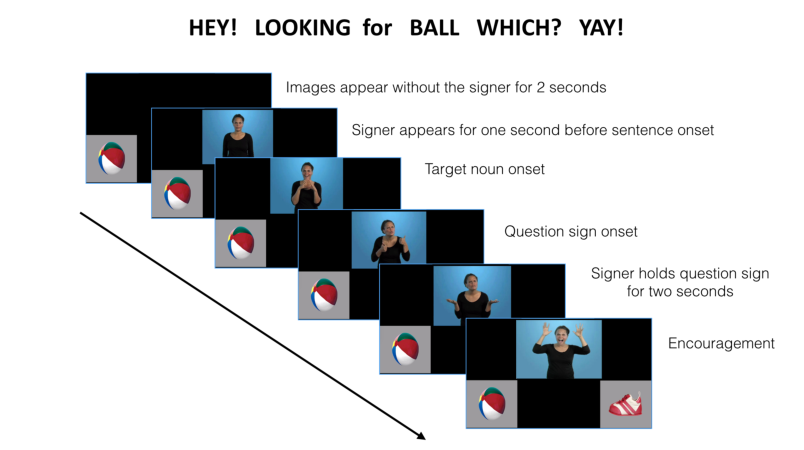
\includegraphics{Figs/timeline-1.pdf}
\caption{Timeline of a trial on the VLP task.}
\end{figure}

\subsubsection{Trial Structure}\label{trial-structure}

Figure 1 shows an example of the stimuli and the timeline of one trial
in the VLP task. On each trial the child saw two images on the screen
for two seconds before the signer appeared. This gave the child time to
explore both images prior to the start of the sentence. Next, children
saw a still frame of the signer for one second, which gave them the
opportunity to orient to the signer prior to the sentence onset. Each
sentence lasted for approximately five seconds and was followed with a
two second ``hold'' that allowed children to shift away from the signer
to the images on the screen. After the hold, the signer gave neutral,
positive feedback to help maintain the child's focus throughout the
task.

\subsubsection{Linguistic and visual
stimuli}\label{linguistic-and-visual-stimuli}

The linguistic stimuli were designed to be comparable to those used in
previous research and to allow for generalization beyond characteristics
of a specific signer and sentence structure. To accomplish this, ASL
stimuli were recorded by two different native ASL-users using two
different but acceptable ASL sentence structures for asking
questions\footnote{See Neidle, Kegl, Bahan, Aarons, \& MacLaughlin
  (1997) for a detailed discussion of the acceptability of these two
  question structures. We analyzed responses for the two sentence frames
  separately and found no significant differences between the two. Thus
  all analyses we report collapse across the two datasets.}:

\begin{itemize}
\itemsep1pt\parskip0pt\parsep0pt
\item
  Sentence-initial wh-phrase: ``HEY! WHERE {[}target noun{]}?''
\item
  Sentence-final wh-phrase: ``HEY! {[}target noun{]} WHERE?''
\end{itemize}

Before each sentence, the signer used a prototypical hand-wave gesture
commonly used in ASL discourse to initiate a linguistic utterance.

Four yoked pairs of eight target nouns (cat---bird, car---book,
bear---doll, ball---shoe) were used. These nouns were selected such that
they would be familiar to most children learning ASL at this age and
have minimal phonological overlap. To prepare the stimuli, a female
native ASL-user recorded several tokens of each sentence, matching them
closely in prosody. These candidate stimuli were then digitized,
analyzed, and edited using Final Cut Pro software. The final tokens were
chosen based on naturalness and prosodic comparability. The mean
duration of target nouns was TODO ms (range = TODO ms). Five filler
trials were interspersed among the 32 test trials (e.g. ``YOU LIKE
PICTURES! MORE WANT?''). Images were digitized pictures presented in
fixed pairs, matched for visual salience with 3--4 tokens of each object
type. Side of target picture was counterbalanced across trials.

\subsubsection{Coding and reliability}\label{coding-and-reliability}

Children's gaze patterns were videotaped and coded frame-by-frame,
yielding a high-resolution record of eye movements aligned with target
noun onset. 25\% of videos were re-coded to assess coder reliability --
agreement within a single frame averaged 98\% on these reliability
assessments.

\subsubsection{Calculating linguistic processing
efficiency}\label{calculating-linguistic-processing-efficiency}

\emph{Accuracy:} Correct looking is a function of the child's tendency
to shift quickly away from the central signer to the target picture in
response to the target sign, and also to remain fixated on the target
picture. To determine the degree to which participants fixated the
appropriate picture across trials, mean proportion looking to target was
calculated for each participant at each 33 ms frame from the onset of
the target noun. Accuracy was defined as the mean proportion of time
spent looking at the target picture out of the total time spent on
either the target picture, the distracter picture, or the signer from
500 to 2000 ms from target noun onset. We selected this window after
looking at the distribution of children's first shifts with the goal of
maximizing the amount of meaningful looking behavior. This window
includes 90\% of children's first shifts off the center signer.
Importantly, the VLP task includes a central signer, which functions as
a central fixation point similar to adult psycholinguistic experiments.
Thus children could produce four different types of responses on a given
trial: (1) signer-to-target shift, (2) signer-to-distractor shift, (3)
signer-to-away shift, (4) no-shift. All four trial types contribute to
accuracy analyses.

\emph{Reaction Time:} Reaction time (RT) corresponds to the latency to
shift away from the signer to the target picture, measured from the
onset of the target sign. Incorrect shifts were not included in the
computation of mean RT. Additionally, responses prior to 500 ms from
noun onset were excluded because few responses occurred before this cut
point, likely because the child did not have enough time to process
sufficient linguistic input and to mobilize an eye movement; responses
slower than 2000 ms were excluded because these delayed looks are less
likely to reflect a response to the target sign (see (Fernald et al.,
2001)). In addition, 8\% of trials were excluded because children never
shifted off the signer. Note that RT can be calculated only on those
trials on which the child is looking at the signer at the onset of the
noun and shifts within the designated time window. Since children vary
in the likelihood that they will shift on a given trial, mean RTs are
based on different numbers of trials across participants (M =13.4
trials, range =3---25). Finally, 5 children were excluded from RT
analyses because their initial shifts were just as likely to be to the
target as to the distractor. This looking behavior provides evidence
that RTs for these children are not a meaningful measure of language
processing.

\section{Results}\label{results}

First we present an overview of performance on the VLP task, showing
that children become faster and more accurate at comprehending familiar
signs as they get older and progress towards adult levels of language
fluency. Then we present analyses of the links between children's
real-time ASL processing skills and productive ASL vocabulary.

\begin{figure}[htbp]
\centering
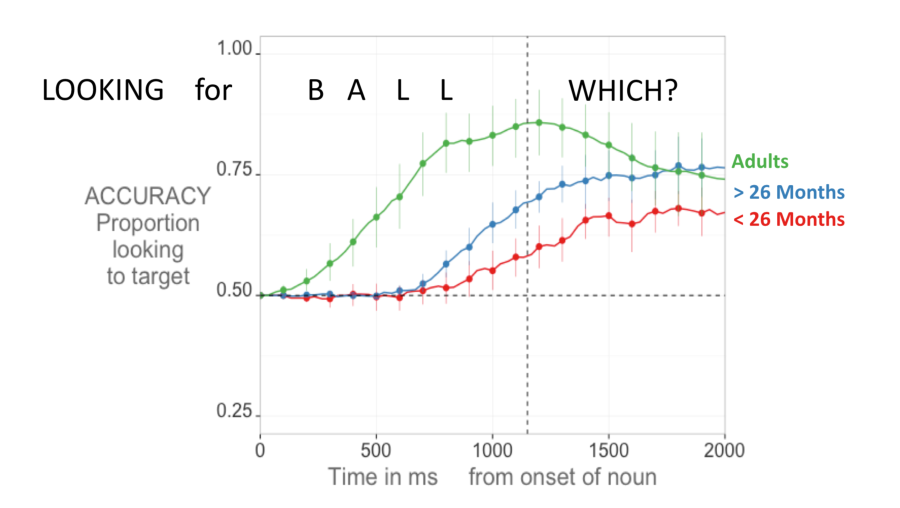
\includegraphics{Figs/profile plot png-1.pdf}
\caption{The timecourse of participants' responses to the target picture
in relation to the unfolding sign for younger children, older children,
and adults. Curves show changes over time in the mean proportion looking
to the correct picture, measured in ms from noun onset; error bars
represent +/- 95\% CI computed by non-parametric bootstrap. The dashed
vertical line indicates mean offset of target noun (TODO ms).}
\end{figure}

\subsubsection{ASL processing
efficiency}\label{asl-processing-efficiency}

Figure 2 provides an overview of the timecourse of correct orienting to
the referent in response to the target sign. The three curves show
changes in the mean proportion of trials on which participants in each
age group fixated the correct referent at every 33 ms interval as the
target sign unfolded. Before seeing the target sign, all participants
fixated on the signer. Interestingly, both adults and children began to
increase their looking to the target picture before the offset of the
target noun, providing evidence that signers were not waiting until the
end of the linguistic utterance to seek out the target image. Children
were slower to respond and less accurate than adults. They maintained
their gaze on the center signer for approximately 700 ms and reached a
lower asymptote. The youngest children took the longest to orient to the
target and were less accurate than both older children and adults.

\emph{Accuracy:} Mean accuracy scores, computed over the 500--2000 ms
window from noun onset, were examined as a function of age. Accuracy was
strongly correlated with age (r(27) = 0.64), indicating that older
ASL-learners were more reliable than younger children in fixating the
target picture.

\emph{Reaction Time:} Mean reaction times were negatively correlated
with age (r(22) = -0.38), indicating that older ASL-learning children
were faster to shift to the target picture than younger ones. Mean
reaction times were also negatively correlated with mean accuracy scores
(r(22) = -0.59) such that those children who were faster to shift to the
target were also more likely to stick on the target image throughout the
analysis window.

Together, the Accuracy and Reaction Time analyses show that signers will
reliably leave a central signer to shift to a target image in the VLP
task, even before the end of the linguistic utterance. Importantly,
signers varied in their response times and accuracy, and this variation
was meaningfully linked to age. Thus, like children learning spoken
language, ASL-learners improve their real-time language processing
skills over the second and third years of life, progressing towards
adult levels of language fluency.

\subsubsection{Links between processing efficiency and ASL
vocabulary}\label{links-between-processing-efficiency-and-asl-vocabulary}

\begin{figure}[htbp]
\centering
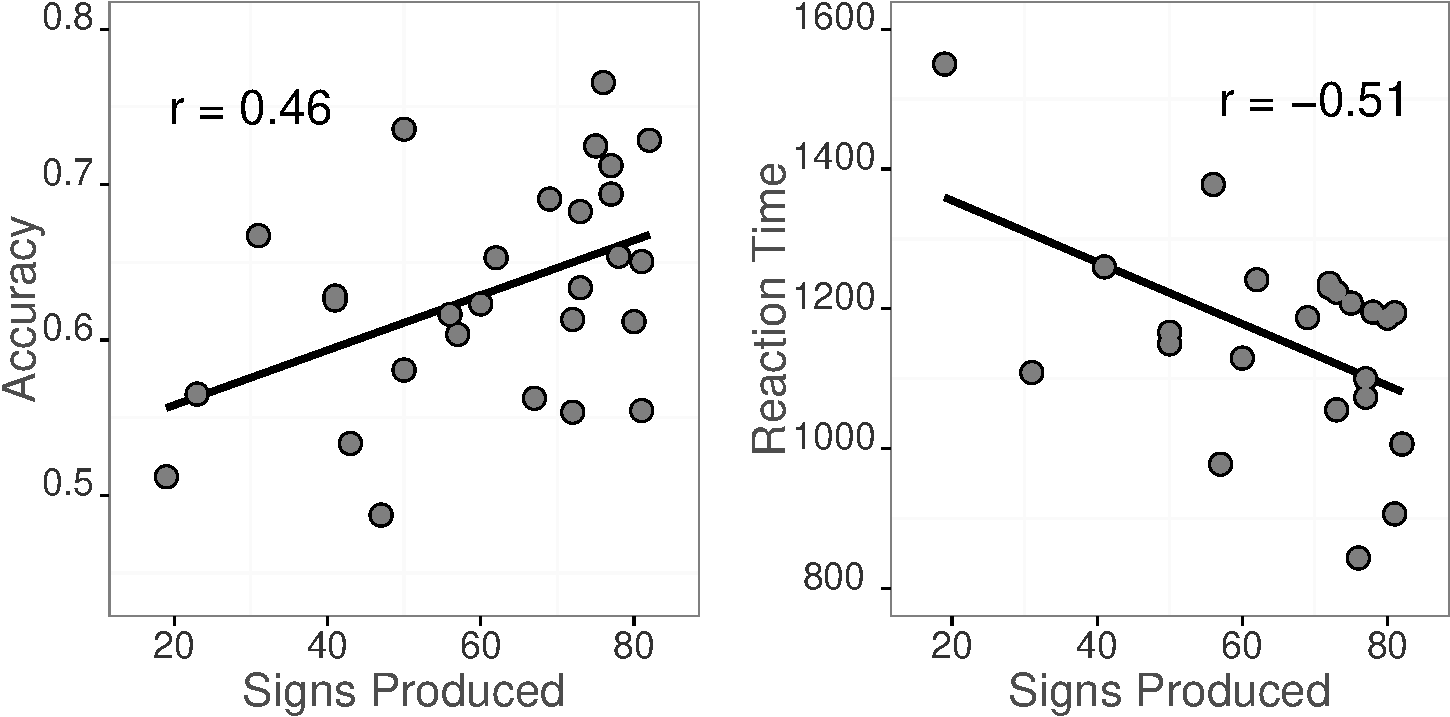
\includegraphics{Figs/vocab scatter plots-1.pdf}
\caption{Relationship between VLP measures and productive ASL
vocabulary. Each data point is an individual child. Panel A shows the
positive relationship between accuracy and vocabulary. Panel B shows the
negative relationship between RT and vocabulary}
\end{figure}

Figure 3 shows the relationships between both VLP processing measures
and children's productive ASL vocabulary. Mean accuracy was positively
related to vocabulary size (r(26) = 0.46) such that children with higher
accuracy scores also had larger productive vocabularies. Mean reaction
times were negatively correlated with vocabulary (r(21) = -0.51)
indicating that children who were faster to recognize ASL signs also had
larger vocabularies.

It is important to point out that age and vocabulary were strongly
intercorrelated in our sample (r(21) = 0.72). In a multiple regression
analysis\ldots{} (TODO: figure out how to talk about regression
analysis)

\section{Discussion}\label{discussion}

Processing words/signs and linking them to objects in real-time is a
fundamental component of language aquisition. ASL-learners must resolve
an apparent conflict between attending to the source of linguistic
information and disengaging to establishing reference. With this study,
we aimed to develop and validate the first measures of young
ASL-learners' real-time language comprehension skills and explore the
links between these skills and both age and vocabulary. There are three
main findings from this work.

First, tracking eye movements during sentence processing is a valid way
to measure young ASL learners' linguistic processing skills. Because
gaze serves a variety of functinos using eye movements as an index of
language skill might not have been possible. For example, proficient ASL
users rely on vision for: (a) processing linguistic information, (b)
looking at objects, (c) regulating turn-taking during conversation
(Baker \& Padden, 1978), and role shifts and direct quotation during
narrative production (Bahan \& Supalla, 1995). Gaze also plays a
syntactic role in ASL, marking pronominal reference and supplementing
manual marking of verb agreement (Metzger, 2002; Neidle, MacLaughlin,
Bahan \& Lee, 2000; Thompson, Emmorey, \& Kluender, 2006). Thus it could
have been the case that measuring eye movements during sentence
processing would not have revealed individual or group differences in
language skills.

Moreover, the VLP task also requires a gaze shift away from the source
of linguistic information to an object on the screen. However, despite
these modality-driven differences we found that ASL-learners exhibit
remarkably similar patterns of looking behavior compared to children
learning spoken language. But children in our study reliably shifted to
the target image as soon as they have enough information, showing the
signature of incremental processing skills thought to be so important
for fluent language comprehension.

Second, like children learning spoken language (Fernald et al., 1998;
Zangl \& Fernald, in press; Zangl et al., 2005), ASL-learners' show
age-related improvement in the efficiency with which they processed
language. All of the target signs were familiar to children in this age
range, yet older children more quickly and accurately identified the
correct referent than younger children. Thus, like children learning
English, young ASL learners showed significant developmental gains in
speech processing abilities over the second and third years of life.

(Discussion about lexical access vs.~learning to disengage from signer)

The third result was the discovery of a link between early ASL
processing skills and children's productive ASL vocabularies. Several
studies have found that English-learning two-year-olds who were
lexically more advanced were also faster and more accurate in spoken
word recognition, even after controlling for age (Fernald et al., 2001,
2006; Zangl et al., 2005). Here we found that ASL-learning children who
knew more signs were also faster and more accurate in speech processing
than those who were lexically less advanced. However, the factors of age
and vocabulary size were highly intercorrelated in this sample and the
majority of the associations between vocabulary and efficiency of spoken
language processing were attributable to variance that was shared
between these two factors. Nevertheless, these results with children
learning ASL were consistent with previous studies with English- and
Spanish- learning children that demonstrate relations between efficiency
in online language comprehension and other concurrent measures of
linguistic achievement.

\section{Acknowledgements}\label{acknowledgements}

We are grateful to the many children and parents who participated in
this research, and to the staff of the California School for the Deaf in
Fremont. Special thanks to Shane Blau, Kat Adams, Melanie Ashland, and
the staff of the Language Learning Lab at Stanford University. This work
was supported by a grant from the

\newpage 

\section*{References}\label{references}
\addcontentsline{toc}{section}{References}

Altmann, G. T., \& Kamide, Y. (1999). Incremental interpretation at
verbs: Restricting the domain of subsequent reference. \emph{Cognition},
\emph{73}(3), 247--264.

Anderson, D., \& Reilly, J. (2002). The macArthur communicative
development inventory: Normative data for american sign language.
\emph{Journal of Deaf Studies and Deaf Education}, 83--106.

Bellugi, U. (1979). \emph{The signs of language}. Harvard University
Press.

Boudreault, P., \& Mayberry, R. I. (2006). Grammatical processing in
american sign language: Age of first-language acquisition effects in
relation to syntactic structure. \emph{Language and Cognitive
Processes}, \emph{21}(5), 608--635.

Carreiras, M. (2010). Sign language processing. \emph{Language and
Linguistics Compass}, \emph{4}(7), 430--444.

Carreiras, M., Guti{é}rrez-Sigut, E., Baquero, S., \& Corina, D. (2008).
Lexical processing in spanish sign language (lSE). \emph{Journal of
Memory and Language}, \emph{58}(1), 100--122.

Corina, D. P., \& Emmorey, K. (1993). Lexical priming in american sign
language. In \emph{34th annual meeting of the psychonomics society}.

Corina, D. P., \& Knapp, H. P. (2006). Lexical retrieval in american
sign language production. \emph{Papers in Laboratory Phonology},
\emph{8}, 213--240.

Dahan, D., \& Tanenhaus, M. K. (2004). Continuous mapping from sound to
meaning in spoken-language comprehension: Immediate effects of
verb-based thematic constraints. \emph{Journal of Experimental
Psychology: Learning, Memory, and Cognition}, \emph{30}(2), 498.

Emmorey, K., \& Corina, D. (1990). Lexical recognition in sign language:
Effects of phonetic structure and morphology. \emph{Perceptual and Motor
Skills}, \emph{71}(3f), 1227--1252.

Fernald, A., \& Marchman, V. A. (2012). Individual differences in
lexical processing at 18 months predict vocabulary growth in typically
developing and late-talking toddlers. \emph{Child Development},
\emph{83}(1), 203--222.

Fernald, A., Perfors, A., \& Marchman, V. A. (2006). Picking up speed in
understanding: Speech processing efficiency and vocabulary growth across
the 2nd year. \emph{Developmental Psychology}, \emph{42}(1), 98.

Fernald, A., Pinto, J. P., Swingley, D., Weinbergy, A., \& McRoberts, G.
W. (1998). Rapid gains in speed of verbal processing by infants in the
2nd year. \emph{Psychological Science}, \emph{9}(3), 228--231.

Fernald, A., Swingley, D., \& Pinto, J. P. (2001). When half a word is
enough: Infants can recognize spoken words using partial phonetic
information. \emph{Child Development}, \emph{72}(4), 1003--1015.

Grosjean, F. (1980). Spoken word recognition processes and the gating
paradigm. \emph{Perception \& Psychophysics}, \emph{28}(4), 267--283.

Hildebrandt, U., \& Corina, D. (2002). Phonological similarity in
american sign language. \emph{Language and Cognitive Processes},
\emph{17}(6), 593--612.

Hurtado, N., Marchman, V. A., \& Fernald, A. (2008). Does input
influence uptake? Links between maternal talk, processing speed and
vocabulary size in spanish-learning children. \emph{Developmental
Science}, \emph{11}(6), F31--F39.

Lew-Williams, C., \& Fernald, A. (2007). Young children learning spanish
make rapid use of grammatical gender in spoken word recognition.
\emph{Psychological Science}, \emph{18}(3), 193--198.

Lieberman, A. M., Borovsky, A., Hatrak, M., \& Mayberry, R. I. (2014).
Real-time processing of aSL signs: Delayed first language acquisition
affects organization of the mental lexicon. \emph{Journal of
Experimental Psychology: Learning, Memory, and Cognition}.

Lillo-Martin, D. (1999). Modality effects and modularity in language
acquisition: The acquisition of american sign language. \emph{Handbook
of Child Language Acquisition}, \emph{531}, 567.

Marslen-Wilson, W., \& Zwitserlood, P. (1989). Accessing spoken words:
The importance of word onsets. \emph{Journal of Experimental Psychology:
Human Perception and Performance}, \emph{15}(3), 576.

Mayberry, R. I., \& Eichen, E. B. (1991). The long-lasting advantage of
learning sign language in childhood: Another look at the critical period
for language acquisition. \emph{Journal of Memory and Language},
\emph{30}(4), 486--512.

Mayberry, R. I., \& Fischer, S. D. (1989). Looking through phonological
shape to lexical meaning: The bottleneck of non-native sign language
processing. \emph{Memory \& Cognition}, \emph{17}(6), 740--754.

Mayberry, R. I., \& Squires, B. (2006). Sign language acquisition.

Newport, E. L. (1990). Maturational constraints on language learning.
\emph{Cognitive Science}, \emph{14}(1), 11--28.

Newport, E. L., \& Meier, R. P. (1985). \emph{The acquisition of
american sign language.} Lawrence Erlbaum Associates, Inc.

Quine, W. (1960). \emph{Word and object}. MIT press.

Snedeker, J., \& Trueswell, J. C. (2004). The developing constraints on
parsing decisions: The role of lexical-biases and referential scenes in
child and adult sentence processing. \emph{Cognitive Psychology},
\emph{49}(3), 238--299.

Tanenhaus, M. K., Spivey-Knowlton, M. J., Eberhard, K. M., \& Sedivy, J.
C. (1995). Integration of visual and linguistic information in spoken
language comprehension. \emph{Science}, \emph{268}(5217), 1632--1634.

Thompson, R., Vinson, D., Fox, N., \& Vigliocco, G. (2013). Is lexical
access driven by temporal order or perceptual salience? Evidence from
british sign language. In \emph{Proceedings of the 35th annual meeting
of the cognitive science society} (pp. 1450--1455).

Zangl, R., \& Fernald, A. (2007). Increasing flexibility in children's
online processing of grammatical and nonce determiners in fluent speech.
\emph{Language Learning and Development}, \emph{3}(3), 199--231.

Zangl, R., Klarman, L., Thal, D., Fernald, A., \& Bates, E. (2005).
Dynamics of word comprehension in infancy: Developments in timing,
accuracy, and resistance to acoustic degradation. \emph{Journal of
Cognition and Development}, \emph{6}(2), 179--208.

\end{document}
